\section{An EKF update using magnetometer measurements}

\subsection{Task 9}

For this segment, I have undertaken a fresh measurement of the magnetic parameters to recalibrate the magnetometer's offset.

The theory of the EKF filter is the same as the accelerometer part, and the function  \texttt{mu\_m} is exactly modified from \texttt{mu\_g}. So I do not derive the kalman filter theory here again.

\subsection{Task 10}

\begin{figure}[H]
 \centering
 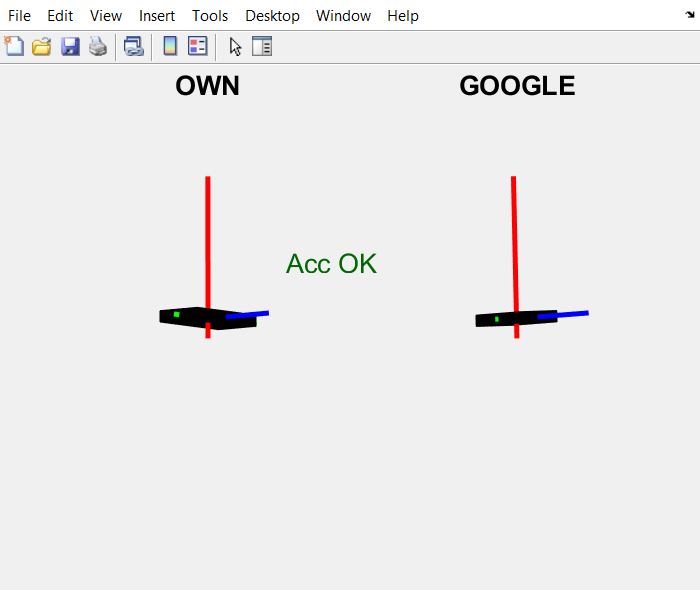
\includegraphics[width=0.6\textwidth]{images/magbegin.png}
 \caption{Begin state with magnetometer added}
 \label{magbegin}
\end{figure}

I gently move and rotate the phone. After the manipulation, the phone ended up in a posture with a certain offset with the real Google one.

After I place the phone exactly beside my computer, the estimated picture of the phone starts to rotate.


\begin{figure}[H]
 \centering
 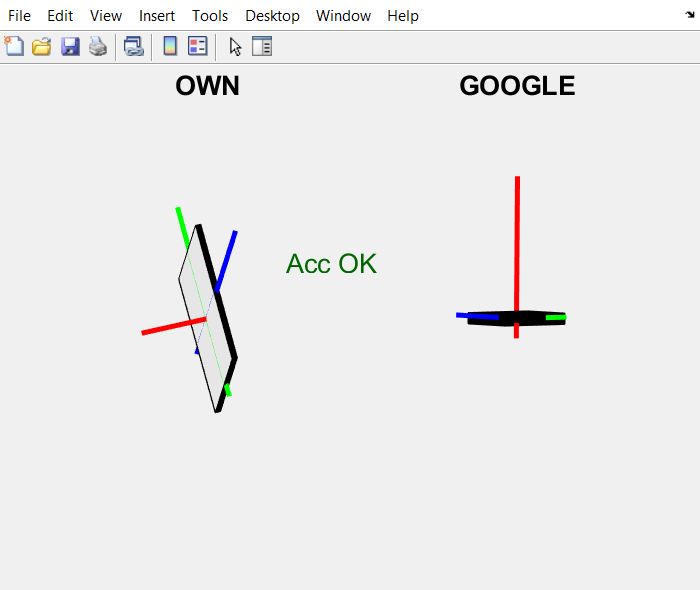
\includegraphics[width=0.6\textwidth]{images/rotatebesidecomputer.png}
 \caption{Place the phone beside the computer}
 \label{rotatemag}
\end{figure}


When I try to return the phone to the operating point, I observed that our filter cannot return to the true state point, and started to swing around it. That is because in the measurement model, we assume the $ f^m_k =0 $, but in reality, this part has a certain value that is attributed to the state $ q_k $, which says our filter now works worse than without using it.

\begin{figure}[H]
 \centering
 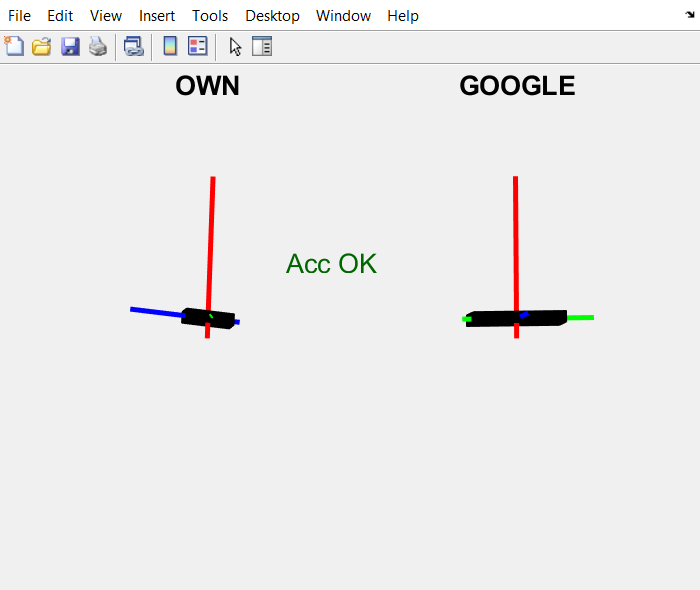
\includegraphics[width=0.6\textwidth]{images/returnmag.png}
 \caption{Return to beginning}
 \label{return}
\end{figure}



\subsection{Task 11}

To construct a basic outlier rejection algorithm, begin by computing the predicted value of $ \hat{L_k} = (1-\alpha)\hat{L_{k-1}}+\alpha \lVert m_k\rVert $. This principle bears a resemblance to a complementary filter.

Then the rejection is set as:
\begin{equation}
    \begin{aligned}
        \lVert m_k - \hat{L_k}\rVert \leq k \cdot \hat{L_k}\nonumber\\
        \text{where  } k = 0.1    
    \end{aligned}
\end{equation}


This formula implies that the update of the magnetometer is only deemed valid when its measured value falls within a narrow range of 10\% around the meticulously predicted value.

When the values of $ \alpha = 0.1 $ and $ L_0 = 0 $ are employed, the phone continues to perform a rotational motion.

\begin{figure}[H]
 \centering
 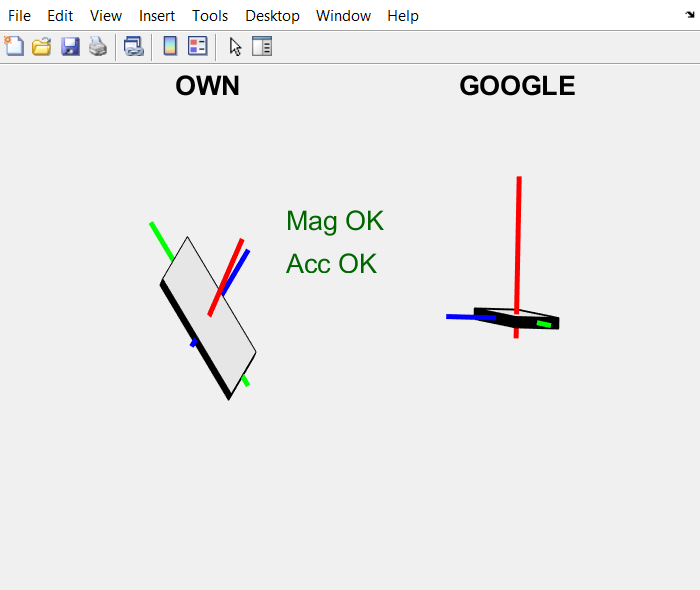
\includegraphics[width=0.6\textwidth]{images/alpha01.png}
 \caption{Set $ \alpha = 0.01 $}
 \label{alpha01}
\end{figure}


When the values of $ \alpha = 0.01 $ and $ L_0 = 0 $ are set, the phone is able to return to its true state and partially alleviate the offset caused by inaccuracies in the accelerometer. However, it still exhibits a sway.

\begin{figure}[H]
 \centering
 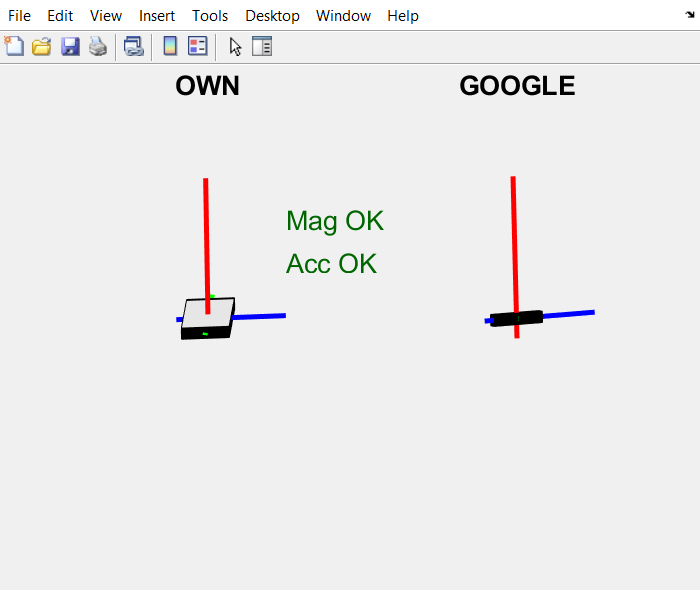
\includegraphics[width=0.6\textwidth]{images/alpha001.png}
 \caption{$ \alpha = 0.01 $}
 \label{alpha001}
\end{figure}

When set  $ \alpha = 0.001 $ and $ L_0 = 0 $, the result holds.

\begin{figure}[H]
 \centering
 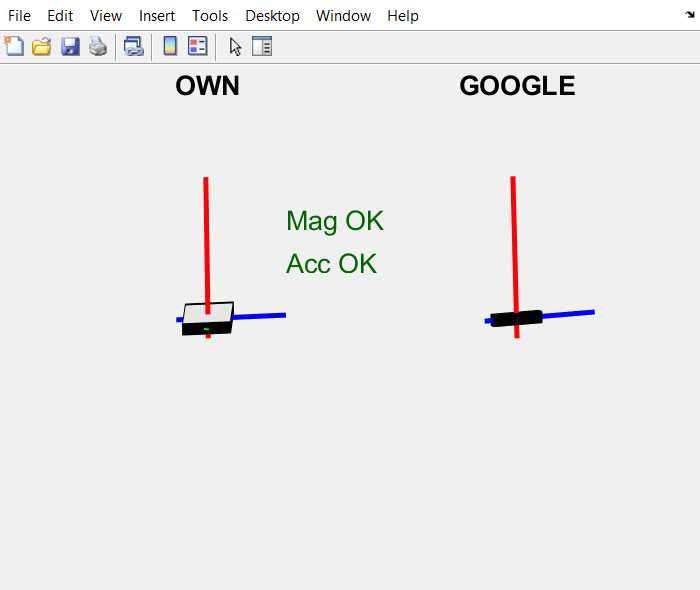
\includegraphics[width=0.6\textwidth]{images/alpha0.01.png}
 \caption{$ \alpha = 0.001 $}
 \label{alpha0001}
\end{figure}

Upon implementing outlier rejection, I observed that when the mobile phone is placed close to a source of interference, specifically my computer, the update of the magnetic state, or "mag" state, is declined. Thus, it effectively eliminates magnetic field interference during movement.

However, considering the algorithm of the AR filter, it is a filtering algorithm based on the previous moment. As long as the phone maintains a particular posture and position for a brief period, it accepts the current magnetometer reading, whatever it is.

Therefore, the underlying assumption of this algorithm is that the phone experiences a sudden magnetic field disturbance from an environment with overall weak background noise, which eventually disappears after a certain duration. This enables the phone to reject the sudden occurrence of magnetic interference. However, it does not distinguish the continuous constant noise unrelated to the Earth's magnetic field.

Hence, when I placed the phone next to the computer, introducing magnetic field interference to test this theory, I did indeed observe that after a while, it started rotating just like it would without the inclusion of outlier rejection.

